\subsubsection{Obfsproxy}
Obfsproxy (obfuscated proxy) \cite{Obfsproxy}, is a client add-on tool written in Python that shapes Tor traffic (between a client and a bridge) to innocent-looking traffic to attempt to circumvent censorship, as censors usually monitor traffic to notice if the client is using Tor (or other similar softwares). 

It works like a proxy, what was cited in section \ref{ssec:toolsBeatCensor} of this document.

\begin{figure}[!ht]
 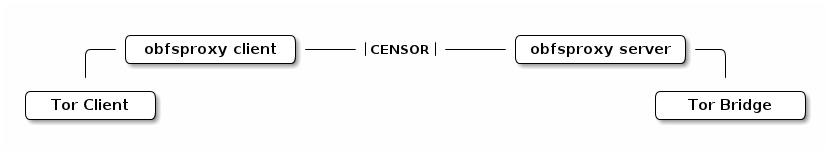
\includegraphics[width=15cm]{obfsproxy_diagram}
 \caption{How Obfsproxy works}
\end{figure}